% Created by tikzDevice version 0.12.6 on 2026-05-17 18:10:24
% !TEX encoding = UTF-8 Unicode
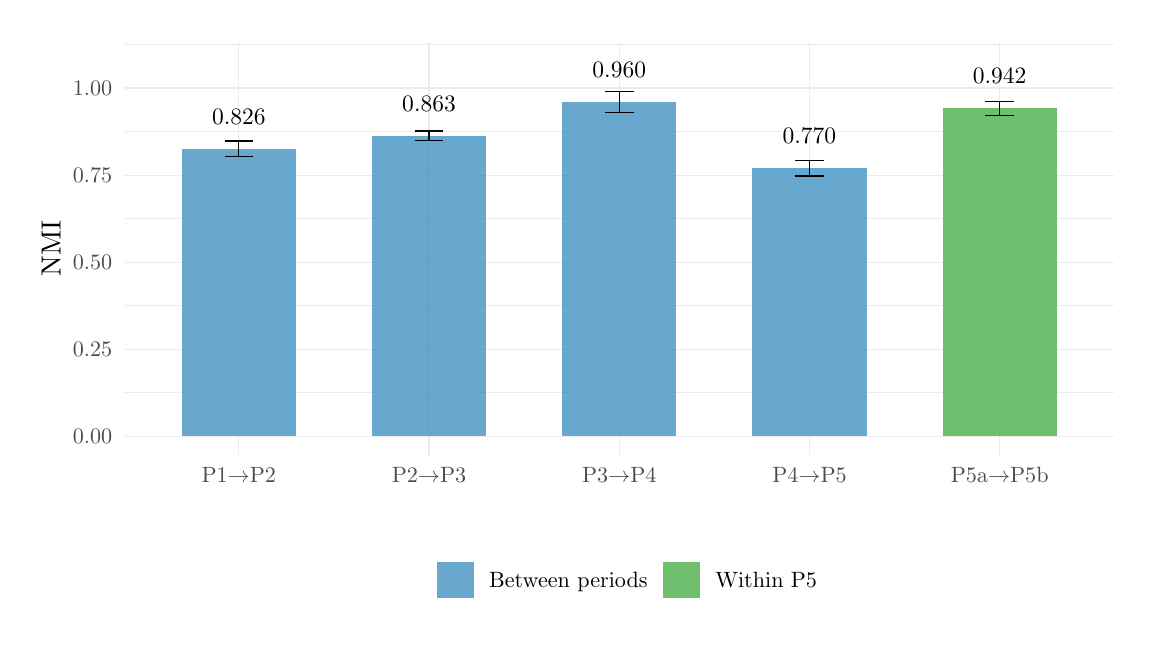
\begin{tikzpicture}[x=1pt,y=1pt]
\definecolor{fillColor}{RGB}{255,255,255}
\path[use as bounding box,fill=fillColor,fill opacity=0.00] (0,0) rectangle (397.48,216.81);
\begin{scope}
\path[clip] (  0.00,  0.00) rectangle (397.48,216.81);
\definecolor{fillColor}{RGB}{255,255,255}

\path[fill=fillColor] (  0.00,  0.00) rectangle (397.48,216.81);
\end{scope}
\begin{scope}
\path[clip] ( 35.05, 62.35) rectangle (392.48,211.81);
\definecolor{drawColor}{gray}{0.92}

\path[draw=drawColor,line width= 0.3pt,line join=round] ( 35.05, 84.87) --
	(392.48, 84.87);

\path[draw=drawColor,line width= 0.3pt,line join=round] ( 35.05,116.32) --
	(392.48,116.32);

\path[draw=drawColor,line width= 0.3pt,line join=round] ( 35.05,147.77) --
	(392.48,147.77);

\path[draw=drawColor,line width= 0.3pt,line join=round] ( 35.05,179.23) --
	(392.48,179.23);

\path[draw=drawColor,line width= 0.3pt,line join=round] ( 35.05,210.68) --
	(392.48,210.68);

\path[draw=drawColor,line width= 0.5pt,line join=round] ( 35.05, 69.14) --
	(392.48, 69.14);

\path[draw=drawColor,line width= 0.5pt,line join=round] ( 35.05,100.60) --
	(392.48,100.60);

\path[draw=drawColor,line width= 0.5pt,line join=round] ( 35.05,132.05) --
	(392.48,132.05);

\path[draw=drawColor,line width= 0.5pt,line join=round] ( 35.05,163.50) --
	(392.48,163.50);

\path[draw=drawColor,line width= 0.5pt,line join=round] ( 35.05,194.95) --
	(392.48,194.95);

\path[draw=drawColor,line width= 0.5pt,line join=round] ( 76.29, 62.35) --
	( 76.29,211.81);

\path[draw=drawColor,line width= 0.5pt,line join=round] (145.03, 62.35) --
	(145.03,211.81);

\path[draw=drawColor,line width= 0.5pt,line join=round] (213.77, 62.35) --
	(213.77,211.81);

\path[draw=drawColor,line width= 0.5pt,line join=round] (282.50, 62.35) --
	(282.50,211.81);

\path[draw=drawColor,line width= 0.5pt,line join=round] (351.24, 62.35) --
	(351.24,211.81);
\definecolor{fillColor}{RGB}{67,147,195}

\path[fill=fillColor,fill opacity=0.80] ( 55.67, 69.14) rectangle ( 96.91,173.06);

\path[fill=fillColor,fill opacity=0.80] (124.41, 69.14) rectangle (165.65,177.72);

\path[fill=fillColor,fill opacity=0.80] (193.15, 69.14) rectangle (234.39,189.92);

\path[fill=fillColor,fill opacity=0.80] (261.88, 69.14) rectangle (303.13,166.02);
\definecolor{fillColor}{RGB}{77,175,74}

\path[fill=fillColor,fill opacity=0.80] (330.62, 69.14) rectangle (371.86,187.65);
\definecolor{drawColor}{RGB}{0,0,0}

\path[draw=drawColor,line width= 0.5pt,line join=round] ( 71.14,175.83) --
	( 81.45,175.83);

\path[draw=drawColor,line width= 0.5pt,line join=round] ( 76.29,175.83) --
	( 76.29,170.29);

\path[draw=drawColor,line width= 0.5pt,line join=round] ( 71.14,170.29) --
	( 81.45,170.29);

\path[draw=drawColor,line width= 0.5pt,line join=round] (139.87,179.48) --
	(150.19,179.48);

\path[draw=drawColor,line width= 0.5pt,line join=round] (145.03,179.48) --
	(145.03,175.95);

\path[draw=drawColor,line width= 0.5pt,line join=round] (139.87,175.95) --
	(150.19,175.95);

\path[draw=drawColor,line width= 0.5pt,line join=round] (208.61,193.69) --
	(218.92,193.69);

\path[draw=drawColor,line width= 0.5pt,line join=round] (213.77,193.69) --
	(213.77,186.15);

\path[draw=drawColor,line width= 0.5pt,line join=round] (208.61,186.15) --
	(218.92,186.15);

\path[draw=drawColor,line width= 0.5pt,line join=round] (277.35,168.78) --
	(287.66,168.78);

\path[draw=drawColor,line width= 0.5pt,line join=round] (282.50,168.78) --
	(282.50,163.25);

\path[draw=drawColor,line width= 0.5pt,line join=round] (277.35,163.25) --
	(287.66,163.25);

\path[draw=drawColor,line width= 0.5pt,line join=round] (346.09,190.17) --
	(356.40,190.17);

\path[draw=drawColor,line width= 0.5pt,line join=round] (351.24,190.17) --
	(351.24,185.14);

\path[draw=drawColor,line width= 0.5pt,line join=round] (346.09,185.14) --
	(356.40,185.14);

\node[text=drawColor,anchor=base,inner sep=0pt, outer sep=0pt, scale=  0.85] at ( 76.29,181.88) {0.826};

\node[text=drawColor,anchor=base,inner sep=0pt, outer sep=0pt, scale=  0.85] at (145.03,186.53) {0.863};

\node[text=drawColor,anchor=base,inner sep=0pt, outer sep=0pt, scale=  0.85] at (213.77,198.74) {0.960};

\node[text=drawColor,anchor=base,inner sep=0pt, outer sep=0pt, scale=  0.85] at (282.50,174.83) {0.770};

\node[text=drawColor,anchor=base,inner sep=0pt, outer sep=0pt, scale=  0.85] at (351.24,196.47) {0.942};
\end{scope}
\begin{scope}
\path[clip] (  0.00,  0.00) rectangle (397.48,216.81);
\definecolor{drawColor}{gray}{0.30}

\node[text=drawColor,anchor=base east,inner sep=0pt, outer sep=0pt, scale=  0.80] at ( 30.55, 66.39) {0.00};

\node[text=drawColor,anchor=base east,inner sep=0pt, outer sep=0pt, scale=  0.80] at ( 30.55, 97.84) {0.25};

\node[text=drawColor,anchor=base east,inner sep=0pt, outer sep=0pt, scale=  0.80] at ( 30.55,129.29) {0.50};

\node[text=drawColor,anchor=base east,inner sep=0pt, outer sep=0pt, scale=  0.80] at ( 30.55,160.74) {0.75};

\node[text=drawColor,anchor=base east,inner sep=0pt, outer sep=0pt, scale=  0.80] at ( 30.55,192.20) {1.00};
\end{scope}
\begin{scope}
\path[clip] (  0.00,  0.00) rectangle (397.48,216.81);
\definecolor{drawColor}{gray}{0.30}

\node[text=drawColor,anchor=base,inner sep=0pt, outer sep=0pt, scale=  0.80] at ( 76.29, 52.34) {P1$\to$P2};

\node[text=drawColor,anchor=base,inner sep=0pt, outer sep=0pt, scale=  0.80] at (145.03, 52.34) {P2$\to$P3};

\node[text=drawColor,anchor=base,inner sep=0pt, outer sep=0pt, scale=  0.80] at (213.77, 52.34) {P3$\to$P4};

\node[text=drawColor,anchor=base,inner sep=0pt, outer sep=0pt, scale=  0.80] at (282.50, 52.34) {P4$\to$P5};

\node[text=drawColor,anchor=base,inner sep=0pt, outer sep=0pt, scale=  0.80] at (351.24, 52.34) {P5a$\to$P5b};
\end{scope}
\begin{scope}
\path[clip] (  0.00,  0.00) rectangle (397.48,216.81);
\definecolor{drawColor}{RGB}{0,0,0}

\node[text=drawColor,rotate= 90.00,anchor=base,inner sep=0pt, outer sep=0pt, scale=  1.00] at ( 11.89,137.08) {NMI};
\end{scope}
\begin{scope}
\path[clip] (  0.00,  0.00) rectangle (397.48,216.81);
\definecolor{fillColor}{RGB}{67,147,195}

\path[fill=fillColor,fill opacity=0.80] (147.94, 10.65) rectangle (161.10, 23.81);
\end{scope}
\begin{scope}
\path[clip] (  0.00,  0.00) rectangle (397.48,216.81);
\definecolor{fillColor}{RGB}{77,175,74}

\path[fill=fillColor,fill opacity=0.80] (229.67, 10.65) rectangle (242.83, 23.81);
\end{scope}
\begin{scope}
\path[clip] (  0.00,  0.00) rectangle (397.48,216.81);
\definecolor{drawColor}{RGB}{0,0,0}

\node[text=drawColor,anchor=base west,inner sep=0pt, outer sep=0pt, scale=  0.80] at (166.75, 14.47) {Between periods};
\end{scope}
\begin{scope}
\path[clip] (  0.00,  0.00) rectangle (397.48,216.81);
\definecolor{drawColor}{RGB}{0,0,0}

\node[text=drawColor,anchor=base west,inner sep=0pt, outer sep=0pt, scale=  0.80] at (248.47, 14.47) {Within P5};
\end{scope}
\end{tikzpicture}
